\documentclass[12pt]{report}
\usepackage[utf8]{inputenc}
\usepackage[T1]{fontenc} 
\usepackage[frenchb]{babel}
\usepackage[official]{eurosym}
\usepackage{amsmath}
\usepackage{graphicx}
\usepackage{wrapfig}
%\DeclareGraphicsExtensions{.pdf,.png,.jpg,.eps}%
\begin{document}

%\includegraphics{elecshock}%

\title{Transmission d'électricité sans fil par le biais de systèmes de transfert d'énergie inductive (IPTS)}
\author{Blaise Ribon, Léo Boudoin, Quentin Boyer}
\date{Janvier 2015}
\maketitle

\begin{abstract}
	Suite a l'expérience menée en 2007 au MIT , nous savons qu'il est possible de transmettre de l'électricité à travers de moyennes distances, de l'ordre de 5m. Ce type de transmissions d'électricité pourrait simplifier les réseaux electriques domestiques étant donné le nombre de câbles demandés par chaque appareil électronique, qui prolifèrent. Mais nous verrons que cette technologie et celles semblables se heurtent à des freins majeurs dans la pratique et que leur mise en place est assez complexe.
\end{abstract}

\tableofcontents

\chapter{Définition et Utilisation de l'electricité} %Titre a changer je pense%
\section{Historique de l'électricité}

\begin{figure}[h!]
  \caption{Le feu dans la préhistoire}
  \centering
	\includegraphics[width=10cm]{feu_prehisoire}
\end{figure}

	    À la Préhistoire déjà, l'Homme a utilisé l'électricité. Par le biais de l'effet Joule, la foudre, en tombant sur le sol, pouvait enflammer des arbres, et parfois créer des incendies dévastateurs. En utilisant ces flammes, les hommes de cette époque onT pu se procurer lumière et chaleur, ainsi qu'une protection efficace contre les prédateurs de l'époque, chose si rare et recherchée qu'elle a donné naissance au mythiques "guerres du feu". Là se résume l'histoire de la domestication de l'électricité pendant des millénaires.
\begin{wrapfigure}{r}{0.3\textwidth}
  \begin{center}
    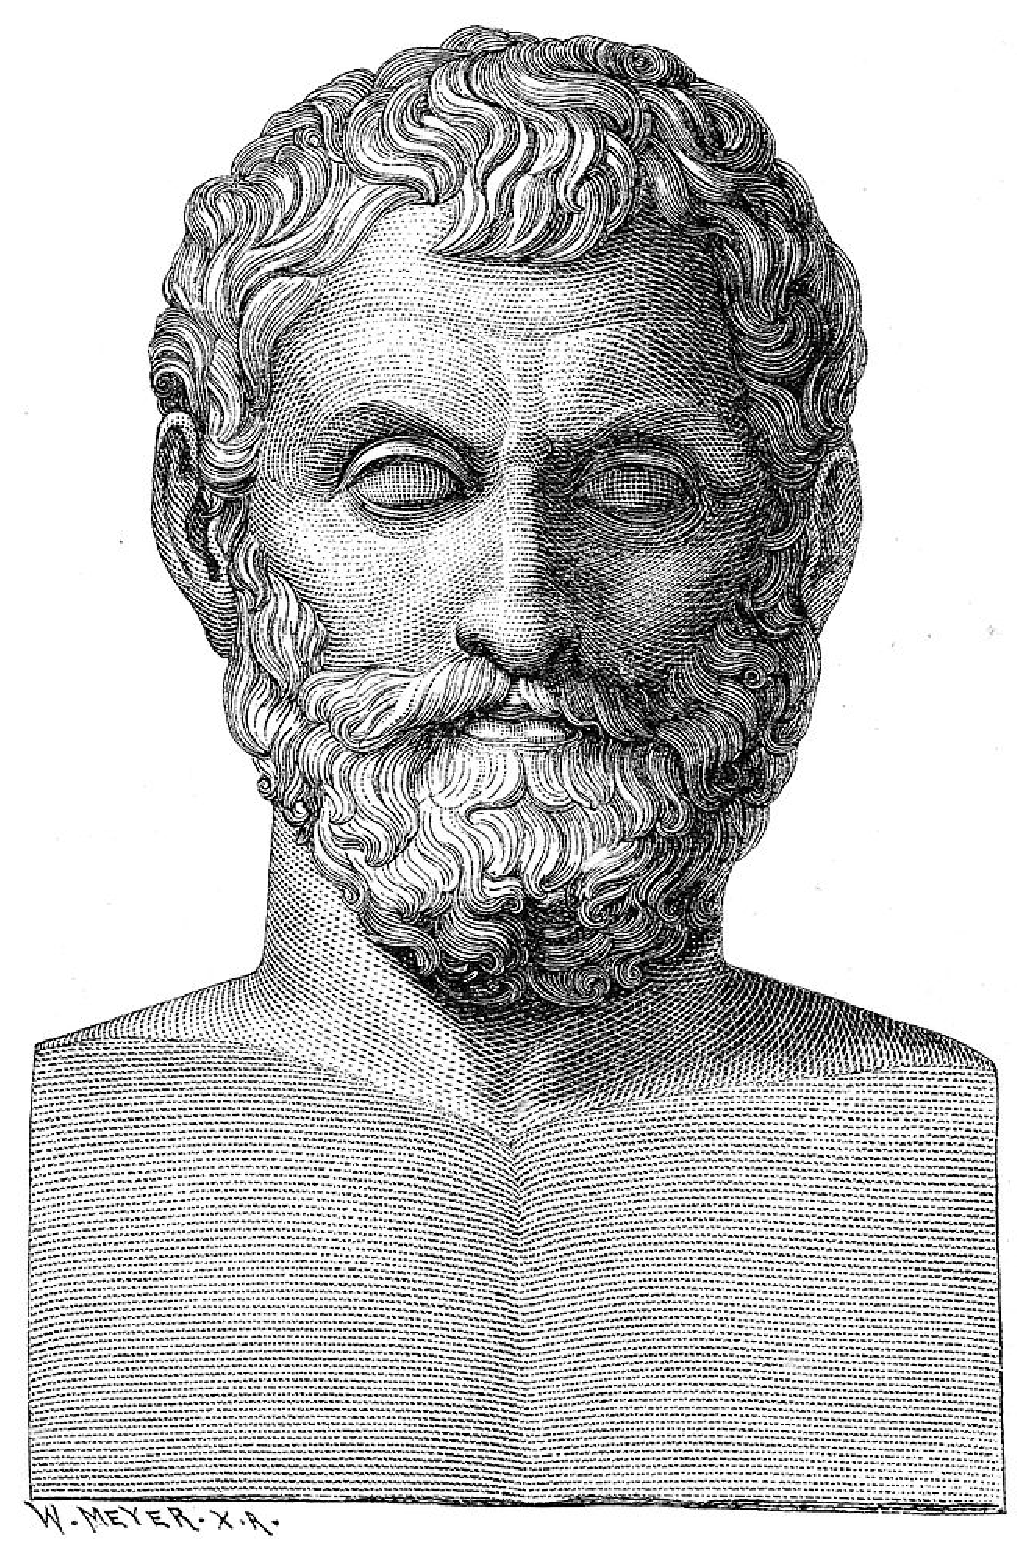
\includegraphics[width=0.225\textwidth]{thales}
  \end{center}
  \caption{Thales}
\end{wrapfigure} Jusqu'au jour où Thalès de Milet(vers 625-vers 547 avant JC), un philosophe grec de l'Antiquité observe le fait que l'ambre jaune, frotté, attire des corps légers comme des brins de paille ou des barbes de plumes. Il baptisera ce phénomène du nom grec de l'ambre jaune, "elektron".

  Ce mot servira plus tard à nommer l'électricité ou tous les phénomènes ayant un rapport. Par la suite, les découvertes se sont succédées lentement juqu'au XVIIIe siècle. On pourra citer la première machine à éléctricté statique d'Otto Von Guericke(1602-1686), constitué d'un simple globe de soufre, ou la classification des corps en fonction de leur comportement, idio-électriques(isolants), et anélectriques(conducteurs), par William Gilbert(1544-1600), qui est le premier à relier électricité et magnétisme.

    Dès 1709 les découvertes s'accélèrent. Francis Hawskbee remplace le globe de soufre de Von Guericke par un cylindre en verre en 1709, et Stephen Grey découvre par hasard que les charges produites par la machine de Hawksbee se déplacent vers le bouchon. Cela amènera, plus tard à la découverte de la portée infinie des charges électriques le long d'un conducteur, avec l'aide de Charles François de Cisternay du Fay. Il découvre aussi que le corps humain est conducteur, et définit deux types d'électricité: la "résineuse"(quand de la résine est frottée) et la "vitreuse"(quand du verre est frotté), qui prépare la découverte de la charge de signes opposés. il créera aussi le premier electroscope connu.

\begin{wrapfigure}{r}{0.45\textwidth}
  \begin{center}
    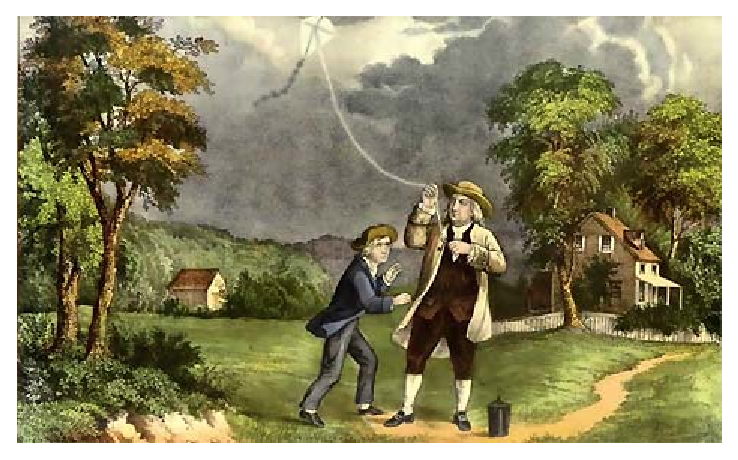
\includegraphics[width=0.4\textwidth]{franklin}
  \end{center}
  \caption{Franklin}
\end{wrapfigure}
De nombreuses autres découvertes ont été faites durant ce siècle, comme les travaux de Benjamin Franklin (1706-1790) avec la mythique expérience où ce scientifique a fait voler un cerf-volant sous un orage(à ne pas reproduire) pour savoir "si les nuages d'où jaillit la foudre sont électrisés ou non", ce qui mènera à la découverte du paratonnerre. Plus tard, Alessandro Volta(1745-1827) multiplie les découvertes dans le domaine de l'électricité. Il crée et améliore de nombreux appareils de mesure électrique, met au point l'électrophore, capable d'accumuler de grandes charges électriques positives, et crée la première pile.

Charles de Coulomb(1736-1806) établira en 1785 la loi homonyme, quantifiant la force électrostatique. Elle définit la force qu'exercent deux charges l'une sur l'autre.
\begin{wrapfigure}{l}{0.3\textwidth}
  \begin{center}
    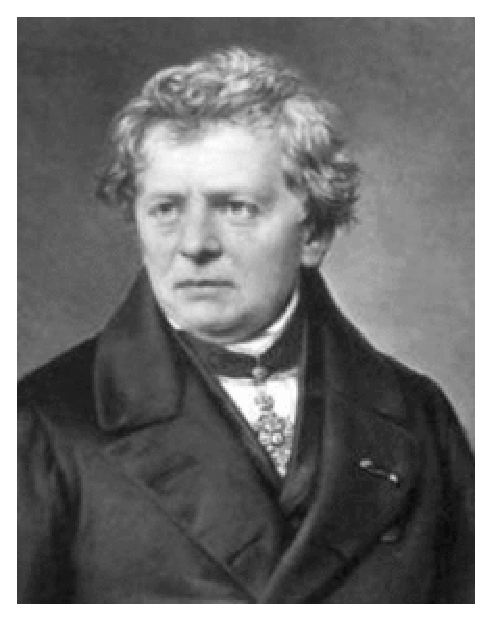
\includegraphics[width=0.25\textwidth]{ohm}
  \end{center}
  \caption{Ohm}
\end{wrapfigure}

Au XIXe siècle, la recherche s'accélère encore. Au début de ce siècle, sir Humphrey Davy(1778-1829) étudie et met au point la première pile à combustible. Sous la férule de Faraday, il créera aussi la première source de lumière électrique, l'arc électrique.


Dans le même temps, Georg Simon Ohm(1787-1854), découvre la résistance des conducturs et etudie les propriétés quantitatives des courants électriques, dont il formule les lois fondamentales. La loi d'Ohm est une relation simple entre l'intensité, la tension, et la résistance \( I = U \times R \) , avec I pour l'intensité, en ampères, U pour les tension, en volts, et R pour la résistance, en Ohms.
    
    En découvrant cette propriété, il affine la notion d'électricité suffisamment pour la rendre utilisable, et ce sera sur cet axe que la recherche scientifique sera orientée dès le second quart du siècle.
\section{Avancées technologiques et Utilisation}
En parallèle commencent les premiers travaux sur l'électromagnétisme, menés par Hans-Christian Oersted(1777-1851), qui découvre le champ magnétique associé à tout courant électrique, et est à la base de la théorie classique de l'électromagnétisme, affinée plus tard par Ampère, Faraday et Maxwell.


André-Marie Ampère (1775-1830) est un physicien, chimiste et mathématicien français est considéré comme un "père fondateur" de l'électromagnétisme. Il introduit la notion de courant, qui aura son nom pour unité, et établit la relation mathématique entre l'intensité et l'orientation du champ magnétique créé par le courant. On lui doit le galvanomètre, le télégraphe électrique, la bobine solénoïde et, en partenariat avec Arago(1756-1853), l'électro-aimant.
Arago, qui découvre les propriété magnétiques du fer placé au centre d'un bobine solénoïde.

\begin{wrapfigure}{l}{0.3\textwidth}
  \begin{center}
    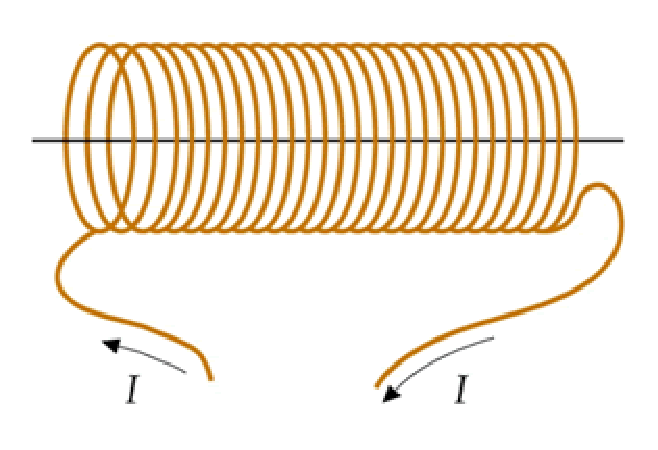
\includegraphics[width=0.25\textwidth]{solenoide}
  \end{center}
  \caption{Solenoide}
\end{wrapfigure}
Michel Faraday(1791-1867) est quant à lui un chimiste et physicien anglais.Il met au point le principe de moteur électrique, et découvre l'induction électromagnétique. Il distinguera aussi les paramagnétiques des diamagnétiques, les bons conducteurs magnétiques étant les premiers, et les mauvais conducteurs les seconds.
Cependant, une part de ses travaux ne seront pas reconnus par ses contemporains.

James Clerk Maxwell fut le premier à s'y intéresser, bien plus tard. Avant son entrée en scène dans le monde scientifique, Peter Barlow met au point sa roue homonyme en 1823, le premier exemple de moteur électrique, et Joseph Henry découvre le phénomène d'auto-inductance, qui permettra de maintenir plus facilement le courant à une valeur donnée. Il mettra aussi au point certains moteurs et un électro-aimant plus simple, outil essentiel pour l'époque.
L'unité d'auto -inductance est nommée le Henry(H) en son nom.

  De nombreux moteurs sont mis au point, comme celui d'un cheval-vapeur de Von Jacobi en 1834, ainsi que des piles, comme la pile à combustible de Grove, en 1839.
  
James Prescott Joule(1818-1889), un physicien amateur, réputé pour son enthousiasme, énoncera la "loi de Joule". Selon cette dernière, un résistor parcouru par un courant électrique reçoit une puissance électrique proportionnelle à la résistance du résistor et au carré de l'intensité du courant. 

Ceci implique que dans un courant électrique, les pertes sont proportionnelles à son intensité et à la résistivité du matériau, et donc inversement à la largeur du câble.

En 1860, un physicien démontre qu'électricité et électromagnétisme ne sont qu'un. considéré comme le plus grand physicien de son époque, James Clerk Maxwell fait énormément avancer la science, en particulier dans la théorie cinétique des gaz, et l'électromagnétisme. Dans ce dernier, il reprend les idées d'Ampère et de Faraday, et met en forme la théorie qui régit les actions à distance.

Zénobe Gramme(1826-1901), un inventeur belge se rend celèbre et rendant possible la création de générateur à courant continu.

Le monde s'éclaire en 1879, grâce à la création des première lampes à incandescence de Thomas Alva Edison(1847-1931). Il s'intéresse aussi au techniques cinématocraphiques, et sera le rival du plus jeune Nikola Tesla.

En 1881, la France organise l'Exposition internationale de l'électricité, qui consacre la naissance de l'électrotechnique. On se souciera également d'unifier les normes. Cette année-là, Edouard Branly réalisera le premier détecteur d'ondes hertziennes.

Nikola Tesla (1856-1943), un ingénieur en électrique yougoslave fonde une société pour la construction des alternateurs en 1887. Ses travaux sur le courant alternatif feront qu'il sera le courant le plus utilisé, à la fois pour le transport et la consommation, dans la mesure du possible, au grand désespoir de Thomas Edison.Il fera un nombre faramineux de découvertes, à tel point qu'aujourd'hui encore on ne sait pas jusqu'où ses travaux sont allés. L'unité magnétique d'induction porte aujourd'hui son nom dans le système SI(le tesla, de symbole T).

\begin{wrapfigure}{l}{0.5\textwidth}
  \begin{center}
    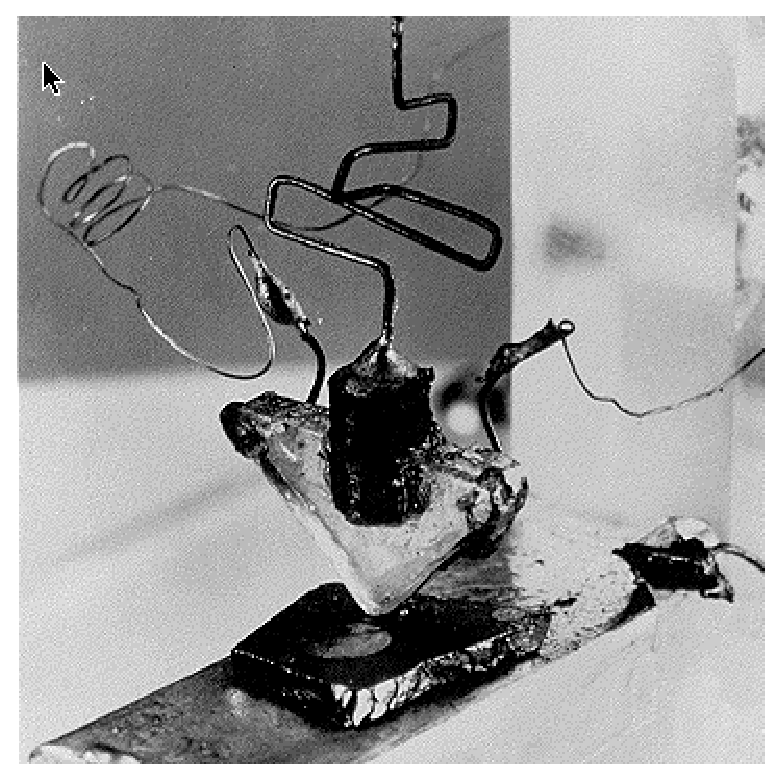
\includegraphics[width=0.4\textwidth]{transistor}
  \end{center}
  \caption{transistor}
\end{wrapfigure} Au début du XXème siècle, les premières émissions radiophoniques et téléphinques ont lieu, et se déveleoppent rapidement.De nombreux société s'orientant sur l'électrique et l'électronique apparaissent, comme Hitachi au Japon, ou la Westinghouse Electric Corporation, aux Etats-Unis
En 1948, le transistor est mis au point par John Bardeen, Walter Brattain et William Shockley dans les laboratoires de la Bell Telephone Company. 

Composant essentiel de l'électronique moderne, il leur vaudra le prix Nobel.
Cette invention sera la dernière révolution que l'électrique, et surtout l'électronique ont connu à ce jour, mais d'autres peuvent être à venir, et même toutes proches. Suite a cette multiplication d'innovations dans l'electricité , celle-ci est devenue une énergie incoutournable dans tout les milieux , domestiques comme industriels mais il reste la question de la transmettre qui est pour le moment assuré par une technologie unique et simple : les câbles. Mais ceux-ci peuvent devenir difficiles à gérer en grand nombre c'est pourquoi nous allons voir si l'on peut \textbf{\underline{transmettre de l'energie sans fil efficacement.}}

\chapter{Solutions techniques liées a la transmission d'electricté.}
  Comme presenté auparavant la technologie utilisée pour transmettre de l'énergie electrique sont les câbles. Mais il existe néanmoins d'autres manieres de transmettre cette energie , notamment les systèmes inductifs ou la transmission par laser et micro-ondes.
  
\section{Analyse fonctionnelle}
  La transmission d'électricité se doit d'ailleurs de répondre a certaines contraintes que nous allons lister ici.
\begin{center}
  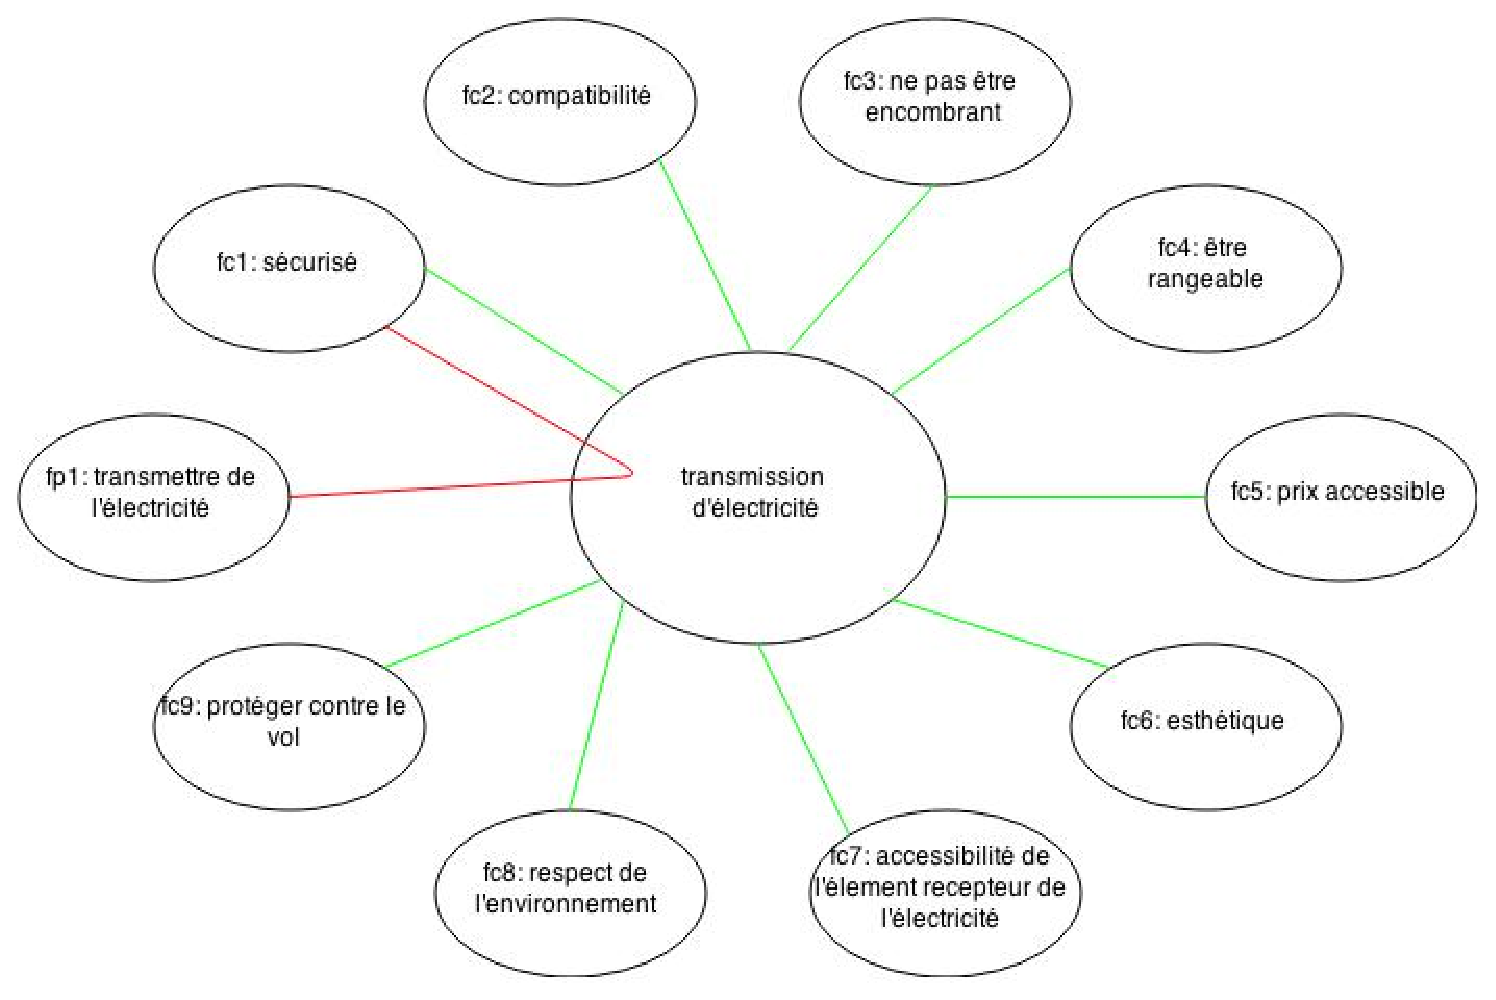
\includegraphics[width=1\textwidth]{pieuvre}
  \underline{Où :} \\
  \begin{tabular}{| l || r |}
  
    \hline
    Fonctions & Description \\
    \hline
    FP1 & Transmettre de l’électricité \\
    FC1 & Ne pas être dangereux pour la santé \\
    FC2 & Compatibilité entre les différentes prises \\
    FC3 & Accessibilité du branchement de l’appareil électrique \\
    FC4 & Avoir un prix accessible \\
    FC5 & Etre agréable à la vue \\
    FC6 & Ne pas être encombrant \\
    FC7 & Possibilité de ranger les émetteurs et les récepteurs \\
    FC8 & Respecter l’environnement \\
    FC9 & Avoir une protection contre le vol \\
    \hline
    
  \end{tabular}
\end{center}
\section{Solution majoritaire actuelle : Les technologies câblées}
\begin{wrapfigure}{l}{0.5\textwidth}
  \begin{center}
    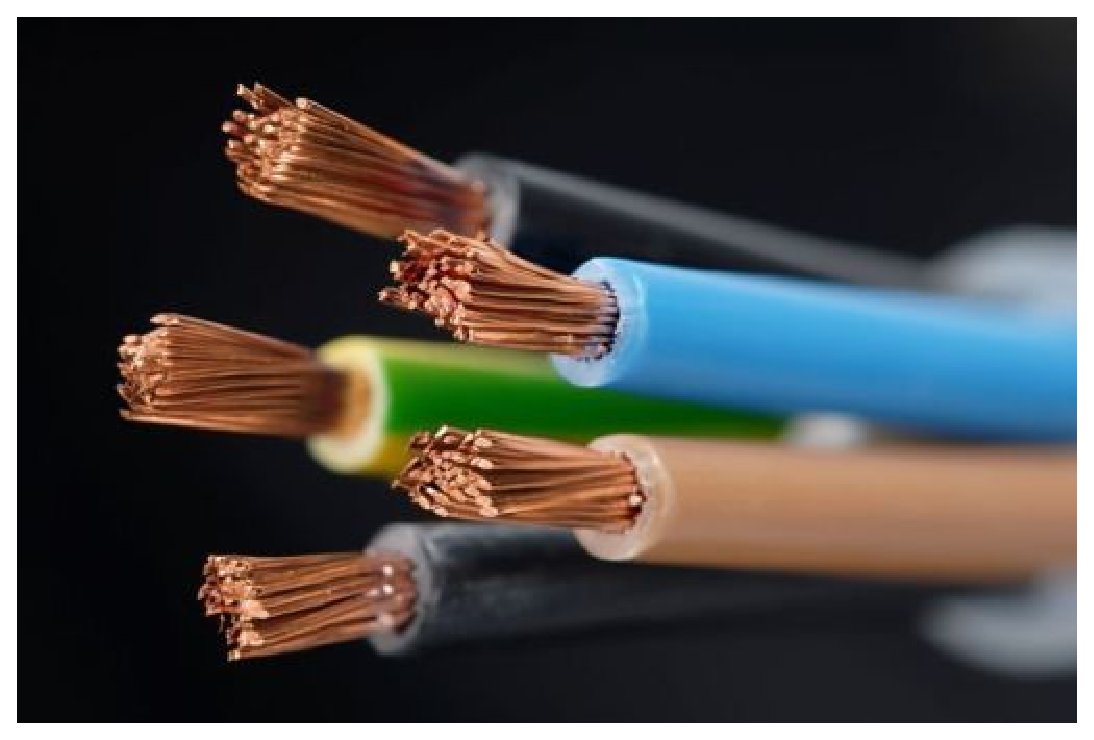
\includegraphics[width=0.4\textwidth]{copperWire}
  \end{center}
  \caption{Fils de cuivre}
\end{wrapfigure} La solution de transmission d'électricité est la plus utilisée au monde, comme dit précedemment , est sans contestation possible le câble électrique , ceci étant dû à un faible coût (jusqu'a 1\$ le mètre), son très haut rendement puisque celui-ci avoisine les 100\% sur les distances courtes avec de faibles puissances. En plus d'être simple , elle n'est pas lourde en terme d'installation puisque les câbles peuvent être facilement mis dans les murs à la construction d'un nouveau bâtiment, être mis dans des gaines si l'on veut en rajouter ensuite et plus simplement on peut utiliser le système des prises pour les appareils temporaires et ponctuels. Grâce à ses avantages incontestables elle est devenue le standard , mais ceci entraîne un probleme non négligable qu'est la densité importante des câbles électriques à proximité des appareils électroniques.
	
	Les matériaux constituant les câbles électriques sont généralement du cuivre pour les longues distances, mais dans les circuitis imprimés on peut utiliser l'or pour sa conductivité électrique extrême, malgré son coût tout aussi élevé, de l'ordre de la dizaine de milliers d'euros le demi kilo. Voici ici un tableau qui récapitule la conductivité de divers métaux plus ou moins utilisés dans les réseaux câblés.

\begin{center}
\begin{tabular}{| l | c | r |}
	\hline
	Matériel & Résistivité électrique en \( n\Omega .m \)& Prix au Kilo \\
	\hline
	Cuivre & 16.78 & 1.08 \euro{}  \\
	Or & 22.14 & 29878 \euro{}  \\
	Fer & 96.1 & (Minerai de fer) 0.07 \euro{}  \\
	Argent & 15.87 & 402 \euro{}  \\
	\hline
\end{tabular}
\end{center}

\begin{wrapfigure}{l}{0.5\textwidth}
  \begin{center}
    \setlength\fboxsep{0pt}
    \setlength\fboxrule{0.5pt}
    \fbox{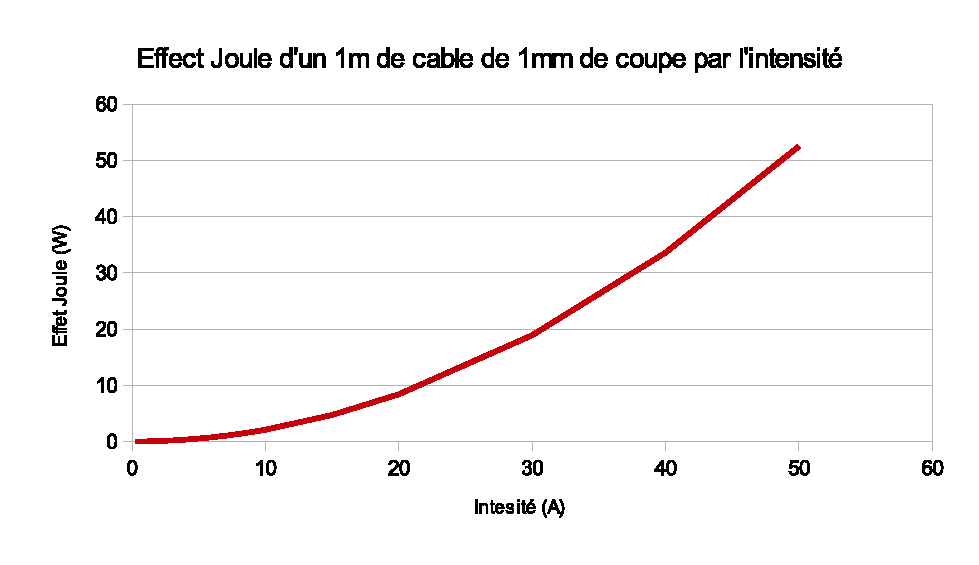
\includegraphics[width=0.45\textwidth]{Joule}}
  \end{center}
  \caption{L'effet joule}
\end{wrapfigure}Un effet négatif important produit par des câbles est l'effet Joule, exprimé dans dans le cadre d'application de la loi d'Ohm par la formule \( P=I^{2} \times R\)\cite{wiki2} ou R est la résistance, liée a la résistivité (\(\rho\)) par la formule \( R= \rho \frac{\ell}{A} \)\cite{wiki3} dans laquelle \(\ell\) est la longeur et A est la surface de coupe en \(m^2\).
D'ou la résistance d'un câble de 1m de long et de 1mm de diamètre est \(17 \times 10^{-9} \times \frac{1}{\pi (0.5 \times 10^{-3})^{2}} = 0.021 \Omega \) et donc l'effet joule produit dans le cas d'un courant de 1A est de \( P=1^{2} \times 0.02 = 0.02 W\).

	Néanmoins d'autres problèmes peuvent occurer dans le cas d'une utilisation domestique , comme la profusion de câbles qui génèrent des nuisances esthétiques et des nuisances magnétiques générées par les câbles nombreux qui subissent le phénomène de diaphonie (ou crosstalk)\cite{wiki4}
\begin{wrapfigure}{r}{0.4\textwidth}
  \begin{center}
    \setlength\fboxsep{0pt}
    \setlength\fboxrule{0.5pt}
    \fbox{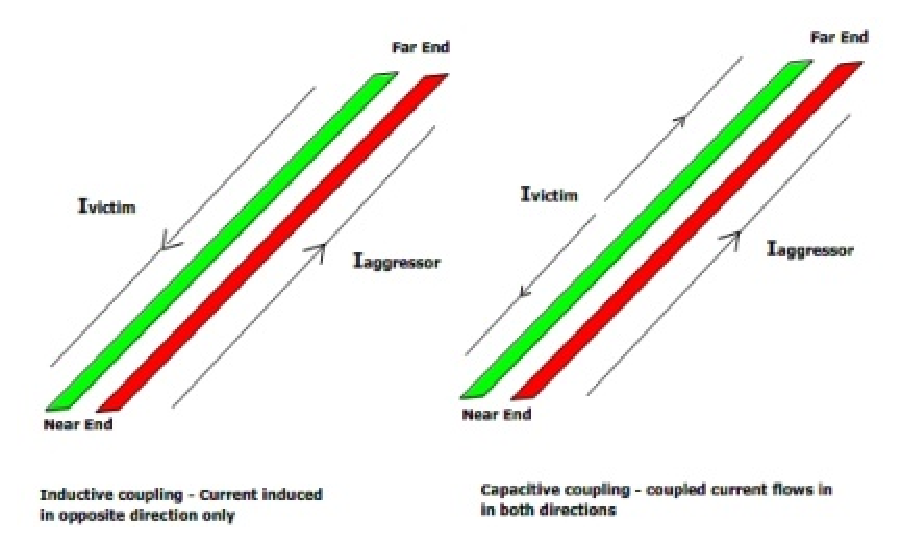
\includegraphics[width=0.3\textwidth]{crosstalk}}
  \end{center}
  \caption{Diaphonie}
\end{wrapfigure}, qui est une interférence entre les signaux passant par un câble dans un câble proche. C'est d'ailleurs pour cette raison que lorsque les signaux transmis sont importants et ne doivent pas etre corrompus on utilise des câbles torsadés,  qui limitent le phenomène. La problématique du transport d'objets électroniques de plus en plus consommateurs mais qui se veulent autonomes se pose, où l'on est obligé de se séparer d'eux pour les recharger ceci empêchant de bénéficier des avantages majeurs de ces objets autonomes , avec comme exemple le cas des téléphones portables , ou la problématique plus importante du rechargement des voitures électriques qui est long, et il ne faut pas oublier de brancher un câble sinon rien n'occure. Les câbles électriques que nous utilisons donc depuis le début de l'utilisation de l'électricité ne sont plus adaptés à un monde qui se veut de plus en plus libéré de toutes les contraintes et de s'affranchir des contraites liés au technolgies filaires , avec comme exemple le développement des téléphones portables ou de la wifi pour pallier la dépendance câblée de l'ethernet. Pour ces raisons et celles que nous allons lister ensuite , les technologies cablées ne semblent pas être la technologie optimale.

	Du point de vue de l'utilisteur , le systeme câblé est relativement lourd pour les raisons suivantes :
\begin{itemize}
	\item chauffe le câble donc rique de surchauffe.
	\item encombrants, s'emmêlent.
	\item problèmes de compatiblités.
	\item problèmes de casse d'un fil.
	\item problèmes d'accessibliliés.
	\item câbles à changer car ils s'abîment.
	D'ou les risques suivants:
	\item risque d'électrocution à cause d'un contact avec un fil dénudé ou abîmé.
	\item risque de surchauffe d'un fil donc d'incendie.
	\item risque de court circuit.
\end{itemize}
\section{Technologies transmetant de l'energie sans-fil \cite{wiki5}}
  \subsection{Les lasers}
\begin{wrapfigure}{r}{0.6\textwidth}
  \begin{center}
    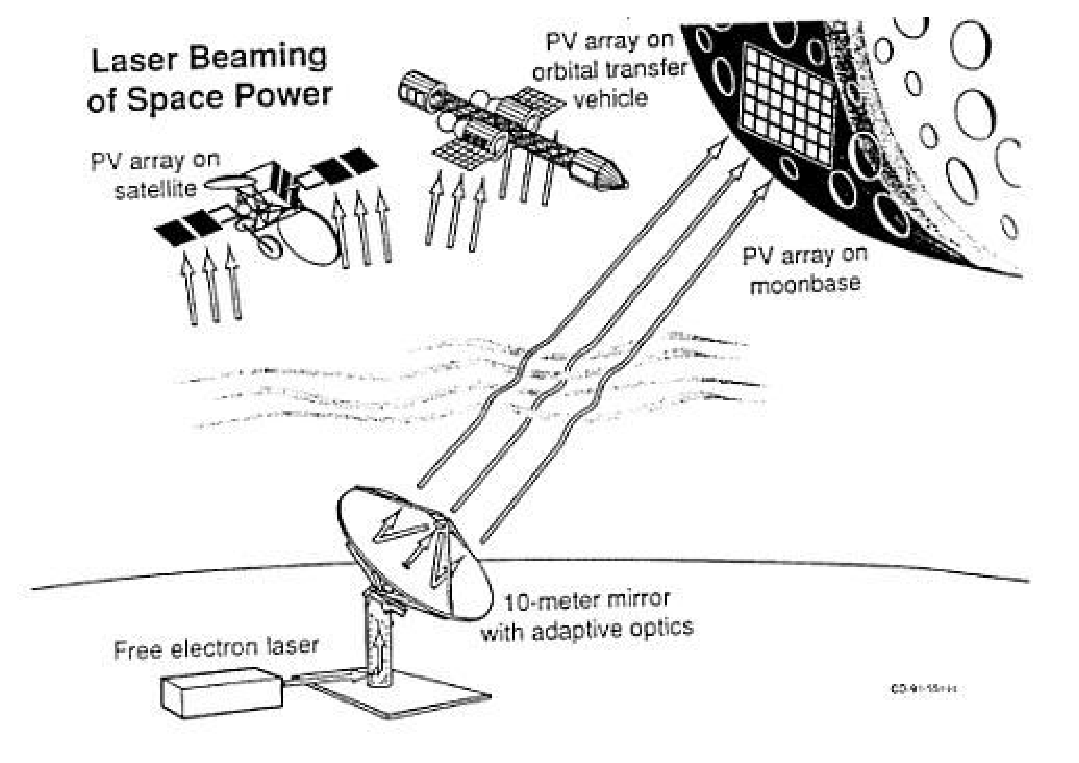
\includegraphics[width=0.5\textwidth]{laser}
  \end{center}
  \caption{Transmission sur de tres longues distances}
\end{wrapfigure}Contrairement a l'idée de transmettre de l'électricité directement grâce au champs magnétiques , l'on peut transmettre cette énergie par les lasers, et la convertir ensuite en électricité par des cellules photovoltaïques. Cette technologie à l'avantage majeur de fonctionner sur des distances beaucoup plus grandes, de l'ordre de quelques kilomètres puisque la dispersion des lasers est moindre et celui ci est uni-directionnel. Le rendement de ce système est aussi légèrement supérieur , puisque la création du lasers est plutôt efficace , et la réception a un rendement de l'ordre de 50\%. Mais ces deux avantages sont compensés par deux inconvénients qui ne gênent pas les champs magnétiques qui sont que cette technologie doit avoir une ligne de vue pour pouvoir fonctionner, et des obstacles comme des arbres qui poussent pourraient interrompre la transmission, et cette dernière peut etre complètement invalidée en cas de pluie ou brouillard.
    \subsection{Les micros ondes}
\begin{wrapfigure}{l}{0.4\textwidth}
  \begin{center}
    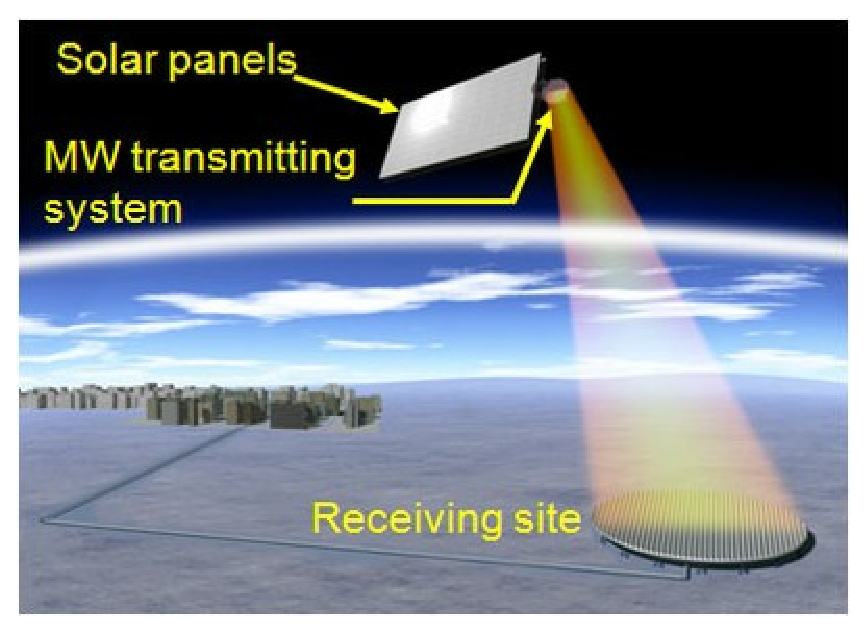
\includegraphics[width=0.3\textwidth]{microwave}
  \end{center}
  \caption{Transmission sur de tres longues distances}
\end{wrapfigure}Dans le même domaine que les lasers l'on peut utiliser les micros-ondes , ce que les hommmes on déjà fait dès les années 1970 à 1990 , qui ont comme avantage d'être bien moins afféctées par les conditions météorologiques, mais ceci est au détriment de la distance, puisque les micros ondes se dispersent beaucoup plus que les lasers, et leurs effets peuvent être plus nocifs sur les êtres humains.

  Néanmoins ces deux techologies sont moins adaptées a un usage domestique puisqu'elles demandent une ligne de vue, mais puisque la seule perte qu'elles subissent dont le réflection et la dispertion , si posssede des antennes très grandes on peut les utiliser pour des transmissions terre-espace.
\subsection{Les technoliges inductives}
  Un autre moyen de transmettre de l'energie sans fil , et dans ce cas directement de l'energie electrique est de passer par les sytemes inductifs , qui ne sont a l'heure actuelle utililsés que dans des tres courtes distances avec deux applications plus ou moins communes domestiques : les brosses a dent sans fil électriques et les systèmes servant a recherger les nokias lumias sans fil. Tout les systèmes inductifs de transfert d'énergie (ou abrégé en anglais par IPTS) fonctionenenet sur le meme principe: un champ magnétique induit par un solénoïde se répercute dans une autre bobine ce qui permet de génerer un courant électrique sans fil avec les-dits champs magnétiques. Néanmoins pour optimiser les systemes IPTS l'on à developpé des variations dans l'application de cette méthode.
Voici les avantages des technologies non câblées:
\begin{itemize}
	\item ne s'emmêle pas.
	\item pas de problèmes de compatibilité.
	\item pas de casse d'un fil.
	\item pas de surchauffe d'un câble .
	\item pas de problèmes d'accessibilité (horloge en hauteur, lumière de sortie de secours).
	\item plus de problèmes d'étanchéité.
	\item pas de câbles à changer.
\end{itemize}
Cette technologie présente néamoins des risques étants :
\begin{itemize}
	\item contact avec une bobine qui transmet l'électricité mais elles seront protégé par un couvercle.
	\item sinon pas de danger si on est dans le genre de champ magnétique comme champs pour le MIT, et l'expérience du KAIST.
\end{itemize}
\section{Comparatif des systèmes de transfert d'énergie.}
	Sans aucun doute possible la technologie actuelle n'est pas la plus pratique puisqu'elle impose de lourdes contraintes , étant donné que l'on en peut pas déplacer les appareils connectés au système , et que ce systeme n'est pas du tout esthetique, critère de plus en plus important maintenant. Quoique cette technologie présente deux aspects techniques importants puisuqe du a sa simplicité elle tombe potentiellement peu en panne et elle a un rendement tres importants comme dit précedemment. Les alternatives à cette technologie monopolisante sont de deux ordres , premièrement on peut utiliser les lasers qui on un avantage énorme de distance puisque l'on pourrait les utiliser entre la terre et la lune , avec un rendement assez peu dépendant de la distance , qui ne depend presque que de la reception car les cellules photovoltaïque on un rendement de l'orde de 50\%. Dans le même ordre d'idée on peut utiliser les micro-ondes , qui ont un rendement supérieur au lasers mais qui est plus lourd à installer comme precisé auparavant. Sachant que ces deux technologies souffrent d'une faille majeure dûe à la ligne de vue demandée pour qu'elles fonctionnent. La troisième technologie présentée semble être le meilleur compromis entre distance , rendement et praticité puisqu'elle ne demande pas de ligne de vue , mais possède pour l'instant un rendement inférieur aux autre technlogies avec l'avantage majeur d'être sans-fil , nous allons donc détailler plus les systèmes IPTS maintenant.

\chapter{Détails des systemes IPTS}
  Suite au choix des technologies ITPS pour transmettre de l'électricté sans fil , nous allons approfondir les raisons de ce choix ici en détaillant plus profondément les technlogies , avec deux variations des systèmes inductifs , l'un qui a commencé a etre développé en 2007, et est maintenant commercialisé sous le nom de "WiTricity" et l'aute qui , étant beaucuop plus récente , n'est pas encore aussi approfondie ni aussi testée que la WiTricity.
\section{Présentation des technologies présentes}
\subsection{Une solution IPTS efficace : Le système de couplage magnétique par résonance (CMRS) \cite{mSojal}}
\begin{wrapfigure}{r}{0.5\textwidth}
  \begin{center}
  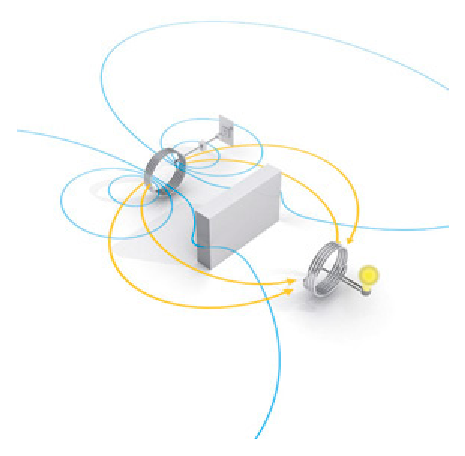
\includegraphics[width=0.4\textwidth]{WTdiagram}
  \end{center}
\caption{Diagramme}
\end{wrapfigure}Le MIT , grâce l'équipe de Marin Soljačić , a développé en 2007 une technolgie inductive utilisant le même pricipe que les transfomateurs électriques ou les brosses a dent électriques. Mais en utilisant des variations de cette technologies cette équipe du MIT a réussi a transmettre de l'énergie a une télévision située de l'autre côté de la pièce , assez pour l'alimenter. Mais le problème de cette technologie est qu'elle est extrêmement dépendante de l'environnement , une petite variation tel le passage d'un être humain , un autre champ magnétique qui perturbe les sytèmes ou une variation de la température ou de l'humidité peut invalider l'expérience. Cette technologie a aussi un incovénient majeur, partagé par tout les systèmes inductifs de transferts d'énergie , plus souvents abrégé en IPTS , qui est le rendement grandement inférieur à un câble électrique déployé sur la même distance. Ceci est dû à la nature même de la technologie qui est un champ magnétique non ou peu dirigé contrairement a un câble électrique où les électrons n'ont que une seule direction possible pour traverser d'un bout a l'autre le système de transmission d'électricité. Néanmoins cette technologie est basée sur la maximisation du rendement possbile par un système IPTS.

	La dépendance aux conditions est dûe au système même : il exploite la resonance magnétique des matériaux , c'est-à-dire la capacité du matériau a produire une réaction énergetique lorsque'il est stimulé par un champ magnétique particulier, ce "champ magnétique de résonance" est affecté par la température , et il est déformé par les obstacles tel qu'un humain. Cette dépendance extrême au champ magnétique est dû au très haut facteur de qualité du système technique utilisés dans l'expérience du MIT , qui ne laisse aucune marge d'erreur dans les fréquences. De plus la mise en place des bobines utilisées pour transmettre de l'électricité demande des réglages complexes où les bobines doivent être accordées pour réagir au bon champ magnétique.
	
\begin{wrapfigure}{l}{0.5\textwidth}
  \begin{center}
    \setlength\fboxsep{0pt}
    \setlength\fboxrule{0.5pt}
    \fbox{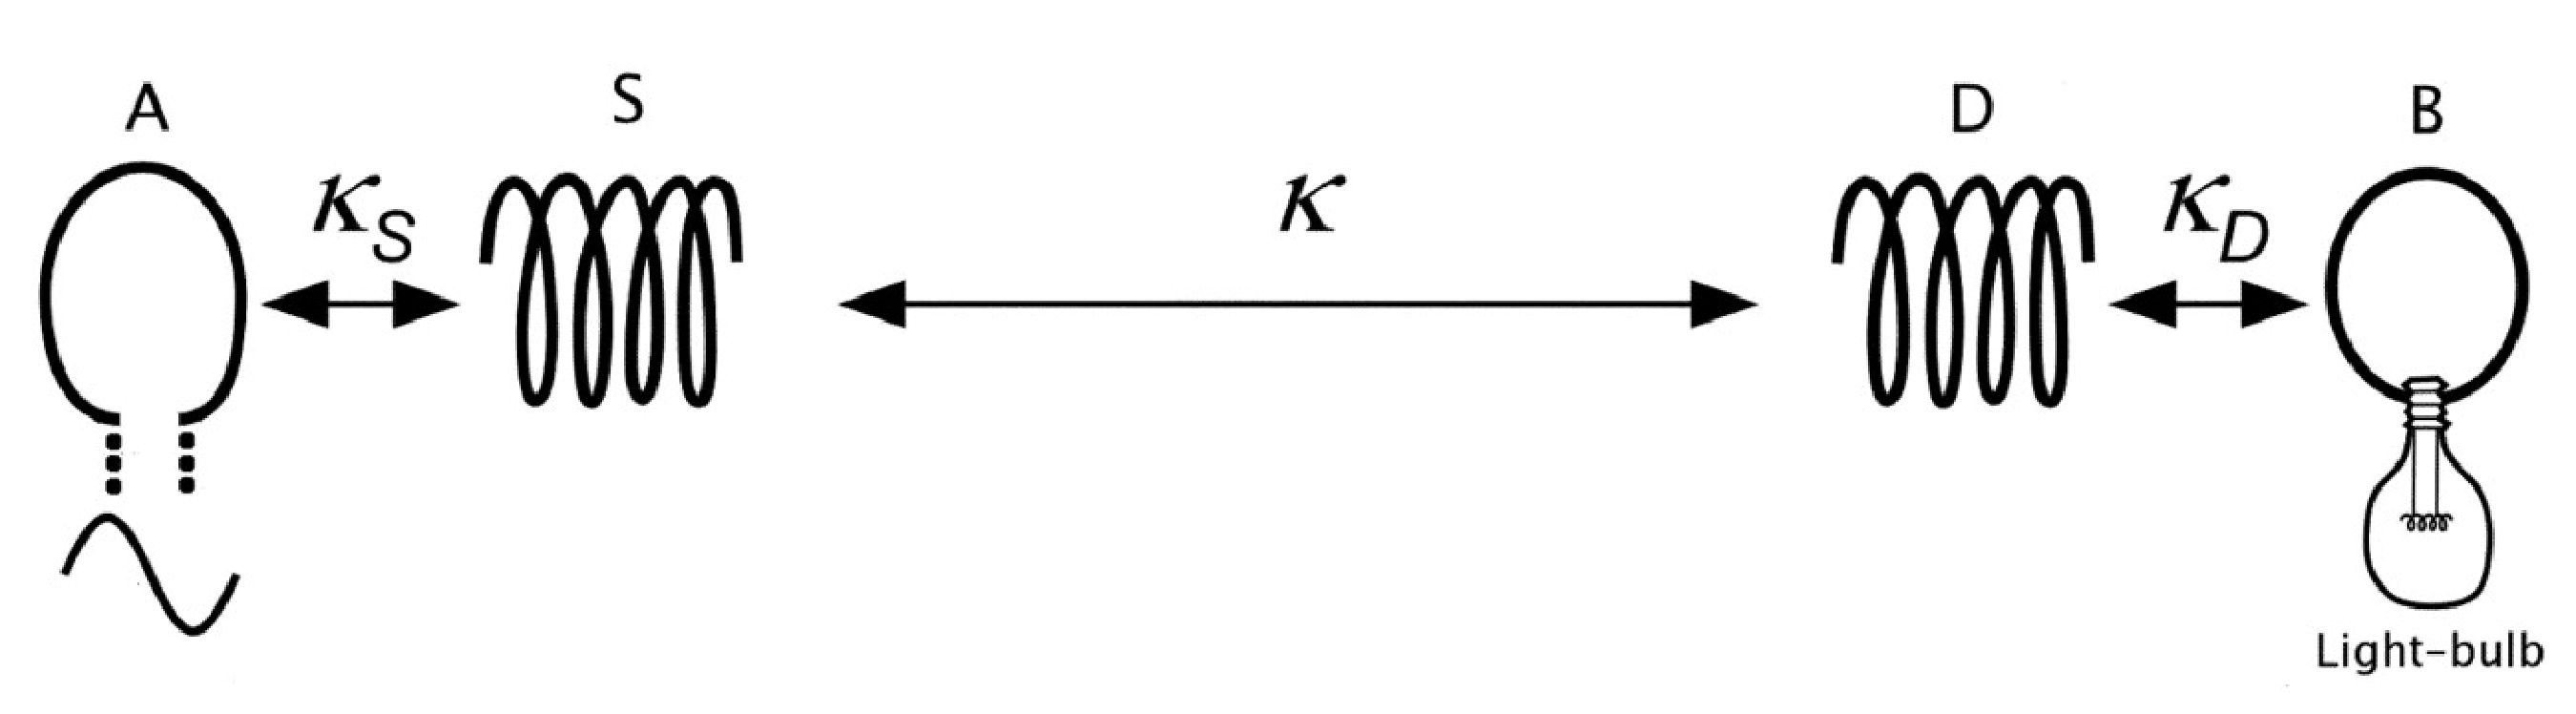
\includegraphics[width=0.45\textwidth]{cmrsMontage}}
  \end{center}
  \caption{Schéma de montage}
\end{wrapfigure} Dans tout IPTS le principe fondamental est identique : Le courant traversant une bobine de fil induit un courant proportionnel dans une autre bobine. Dans la technologie ici présentée ces deux bobines doivent être alignées coaxialement. L'entrée et la sortie sont effectuées via des boucles , et celle d'entrée A doit etre positionnée de telle manière qu'elle n'interfère pas avec la bobine D , l'influence de B sur S étant minimale.

  Cette technologie ne présente d'ailleurs que très peu de danger \cite{wiki1} sur l'être humain , étant donné que ces champs magnétiques n'interagissent pratiquement pas avec les être vivants , de même que le reste de l'environnement d'où la ligne de vue entre les bobines S et D n'est pas nécessaire.
 D'apres Marin Soljačić cette technolgie à du potentiel puisque il a créé une compagnie , WiTricity , pour promulguer sa découverte et il croit que cette technologie pourrait etre largement utilisée dans le cas de transfert de petites quantités d'énergie comme recharger des téléphones. 7 ans apres cette technologie ne s'est pas énorment démocratisée meme si en 2011 Toyota a investi dans cette compagnie.
\subsection{Une solution IPTS assez fiable : Une transmission utilisant des solénoïdes parallèles\cite{kaist14}}
Contrairement au CMRS ou l'on pensait principalement à l'efficacité et au rendement , faisant des bobines dépendantes des conditions et plus adaptées à transmettre des petites quantités d'énergie , étant donné la complexité de la chose , les chercheurs du KAIST (Korea Advanced Institute of Science and Technology) en partenariat avec le département nucléaire de Corée du Sud ont développé une technologie basée sur des solénoïdes parallèles qui est presque indépendante des conditions , grâce à un facteur qualité tres bas (\(\sim100\) , contrairement au CMRS qui avoisinait les 2000) et une technlogie plus simple à mettre en oeuvre , puisque la réponse n'est pas liée a des fréquences tres spécifiques , mais un peu plus larges.
  
  Cette technologie , étant soutenue par le département nucléaire , à pour vocation de servir d'alimentation de secours dans le cadre de centrales nucléaires , ou le CMRS hyper-sensible ne convient pas , se veut de transmsetre des quantités d'energie largement supérieures à celles prévue par Marin Soljačić. Pour pouvoir achever cet aspect ils ont eu recours à des fréquences largement inférieures au MIT qui utilisait du 9.9 MHz alors que le KAIST utilise des fréquences de 20 kHz , qui est la raison de la baisse du facteur qualité.
  
\begin{wrapfigure}{r}{0.5\textwidth}
  \begin{center}
    \setlength\fboxsep{0pt}
    \setlength\fboxrule{0.5pt}
    \fbox{\includegraphics[width=0.4\textwidth]{coreenMontage}}
  \end{center}
  \caption{Montage}
\end{wrapfigure}Ici le sytème est consitué de deux barres de ferrite parrallèles sur lesquelles sont enroulés 30 fois un fil , cette configuration étant due au peu de place disponible dans les centrales nucléaires et prend moins de place que le CMRS. Ces barres ont des dimension modulables proportionnelement , tout comme le nombre de tours N. L'entrée est gérée par un \{Power Inverter\} et la sortie est presque utlisable telle quelle comme montré par le schéma électrique qui suit.
\begin{figure}
  \begin{center}
    \includegraphics[width=7cm]{diagramC}
  \end{center}
  \caption{Diagramme}
\end{figure}

  Cette technologie est d'ailleurs beaucoup plus efficace lorsque l'on utilise de grande quantités d'énergie , étant donné que la puissance fournie n'est pas proportionnelle a l'intensité du système , mais s'accroît de plus en plus , comme montré dans la figure 3.8. Ceci encore découle de la difference d'applications entre les deux technologies sans fil que nous avons présenté.
\begin{wrapfigure}{r}{0.3\textwidth}
  \begin{center}
    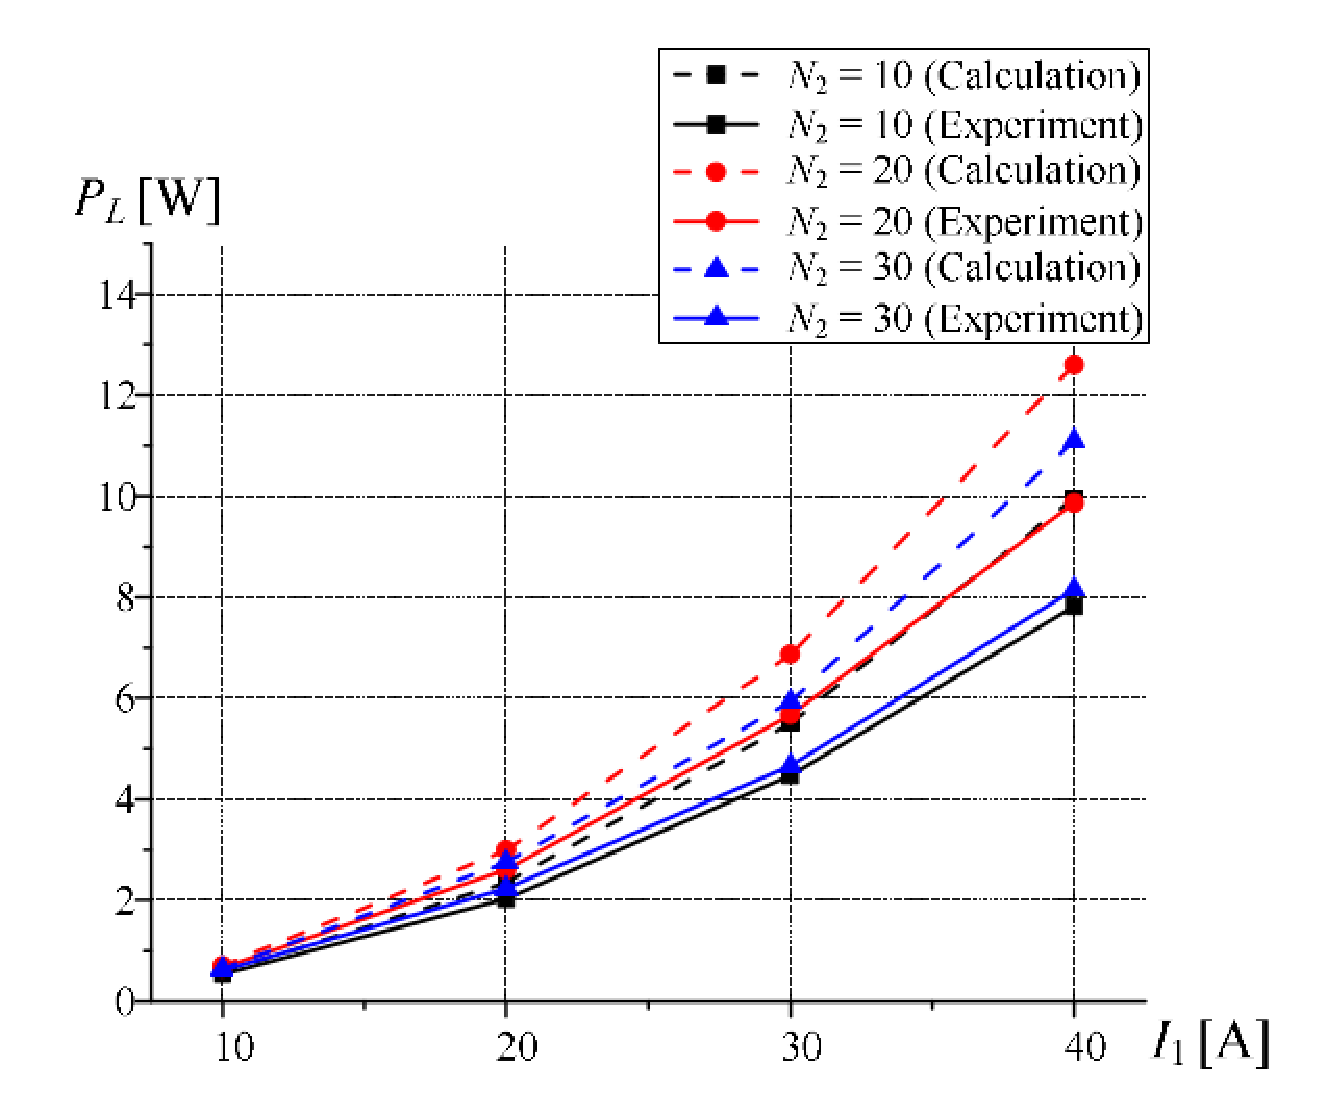
\includegraphics[width=0.2\textwidth]{PparI}
  \end{center}
  \caption{Puissance par intensité}
\end{wrapfigure}

  Contrairement au CMRS qui a eu le temps de se développer , cette technologie ayant étée présentée en 2013 , n'a pas pu être exploitée ni testée , et par conséquent nous ne pouvons comparer objectivement ces deux technologies.
\section{Avantages et limitations des technologies étudiées}
  Les différentes technologies répondent à une même problématique: transférer de l'énergie. Mais les deux solutions sans fil que nous avons étudiées essayent de pallier le problème que les câbles électriques rencontrent de plus en plus , vu leur prolifération active dans les milieux ou l'élecricité est présente. Ils ont aussi les inconvénients de subir l'effet Joule qui peut devenir assez important, impactant aussi le rendement des câbles qui réduit avec la chaleur , qui sinon est proche de 100\%.

  Comme technologie sans fil , le CMRS répond à cette limitation du nombre de câbles importants en les supprimants presque totalement, excluant les entrées, ceux constituants le systeme et la sortie , étant invisbles à l'utilisateur. Mais cet aspect important est en partie eclispé par le rendement inférieur de moitié aux câbles , et à la dépendance du système aux conditions de l'environnement , même si son créateur pense que cet aspect est négligeable puisqu'il a l'intention de produire sa technologie à grande échelle.
  
  L'autre systeme IPTS que nous avons étudié est la technologie du KAIST qui présente elle l'avantage par rapport au CMRS d'une dépendance moindre aux conditions de l'environnement, au détriment d'un rendement encore inférieur , mais cette technologie n'a pas encore pu être testée, ce qui est dû à sa decouverte très récente, il y a seulement 1 an.
  
  Ces deux systèmes ont l'avantage de pouvoir être actif sans ligne de vue, tant qu'aucun matériau altérant le champ magnétique produit n'est situé entre l'émetteur et le récepteur , conduisant à une simplification possible du système électrique domestique, où les prises murales auraient disparu et tout les appareils électriques que nous possédons actuellement seraient parfaitement mobiles à l'intérieur de notre espace domestique.
  
\begin{thebibliography}{9}
    
  \bibitem{mSojal}
  MIT,
  \emph{Wireless Power Transfer via Strongly Coupled Magnetic Resonances},
  2007.

  \bibitem{kaist14}
  KAIST,
  \emph{7m-off-Long-Distance Extremely Loosely Coupled Inductive Power Transfer Systems Using Dipole Coils},
  2014.
  
  \bibitem{wiki1}
  Wikipedia,
  \emph{Resonant inductive coupling}.
  
  \bibitem{wiki2}
  Wikipedia,
  \emph{Joule Heating}.
  
  \bibitem{wiki3}
  Wikipedia,
  \emph{Electrical resistance and conductance}.
  
  \bibitem{wiki4}
  Wikipedia,
  \emph{Crosstalk}.
  
  \bibitem{wiki5}
  Wikipedia,
  \emph{Wireless Power}.
  
\end{thebibliography}
\end{document}
